\documentclass[12pt, twoside]{book}

\usepackage[a4paper,top=2.5cm,bottom=2.5cm,left=3.5cm,right=2cm]{geometry}
\usepackage[utf8]{inputenc}
\usepackage[T1]{fontenc}

\usepackage[slovak]{babel}

\linespread{1.25}

\usepackage{listings}
% ukazky kodu su cislovane ako Listing 1,2,...
% tu je Listing zmenene na Algoritmus 1,2,...
\renewcommand{\lstlistingname}{Algoritmus}
\lstset{frame=lines}

\usepackage{graphicx}
\usepackage{pdfpages}
\usepackage{url}
\usepackage{xurl}
\urlstyle{same}
\usepackage[hidelinks,breaklinks]{hyperref}

% tikz
\usepackage[dvipsnames]{xcolor}
\usepackage{forest}
\usepackage{colortbl}
\usepackage{tikz}
\usetikzlibrary{positioning, arrows.meta, calc, decorations.pathreplacing}

\usepackage{enumitem}
\usepackage{dirtytalk}
\usepackage{makecell}
\usepackage{multirow}
\usepackage{tabularx}
\usepackage{csquotes}
\usepackage{subcaption} 


\definecolor{rootgray}{HTML}{888780}
\definecolor{nodegray}{HTML}{D3D1C7}
\definecolor{nodetextgray}{HTML}{444441}
\definecolor{teal600}{HTML}{0F6E56}
\definecolor{teal100}{HTML}{9FE1CB}
\definecolor{purple600}{HTML}{534AB7}
\definecolor{purple100}{HTML}{CECBF6}
\definecolor{coral600}{HTML}{993C1D}
\definecolor{coral100}{HTML}{F5C4B3}
\definecolor{ocean}{HTML}{4ba3fa}
\definecolor{oceanborder}{HTML}{0D4F8C}


\def\mfrok{2026}
\def\mfnazov{Systém na podporu analýzy rizík}
\def\mftyp{Diplomová práca práca}
\def\mfautor{Bc. Anton Kica}
\def\mfskolitel{doc. RNDr. Daniel Olejár, PhD.}

\def\mfmiesto{Bratislava, \mfrok}

\def\mfodbor{ Informatika }
\def\program{ Informatika }

\def\mfpracovisko{Katedra informatiky}

\begin{document}     
\frontmatter
\pagestyle{empty}

% -------------------
% --- Obalka ------
% -------------------

\begin{center}
\sc\large
Univerzita Komenského v Bratislave\\
Fakulta matematiky, fyziky a informatiky

\vfill

{\LARGE\mfnazov}\\
\mftyp
\end{center}

\vfill

{\sc\large 
\noindent \mfrok\\
\mfautor
}

\cleardoublepage
% --- koniec oIT-Grundshutz Kompendium [GSK], katalóg modulov pre rozličné oblastibalky ----

% -------------------
% --- Titulný list
% -------------------


\noindent

\begin{center}
\sc  
\large
Univerzita Komenského v Bratislave\\
Fakulta matematiky, fyziky a informatiky\usetikzlibrary{positioning, arrows.meta, calc, decorations.pathreplacing}

\vfill

{\LARGE\mfnazov}\\
\mftyp
\end{center}

\vfill

\noindent
\begin{tabular}{ll}
Študijný program: & \program \\
Študijný odbor: & \mfodbor \\
Školiace pracovisko: & \mfpracovisko \\
Školiteľ: & \mfskolitel \\
\end{tabular}

\vfill


\noindent \mfmiesto\\
\mfautor

\cleardoublepage
% --- Koniec titulnej strany


% -------------------
% --- Zadanie z AIS
% -------------------
% v tlačenej verzii s podpismi zainteresovaných osôb.
% v elektronickej verzii sa zverejňuje zadanie bez podpisov
% v pracach v angličtine anglické aj slovenské zadanie

\newpage 
\setcounter{page}{3}
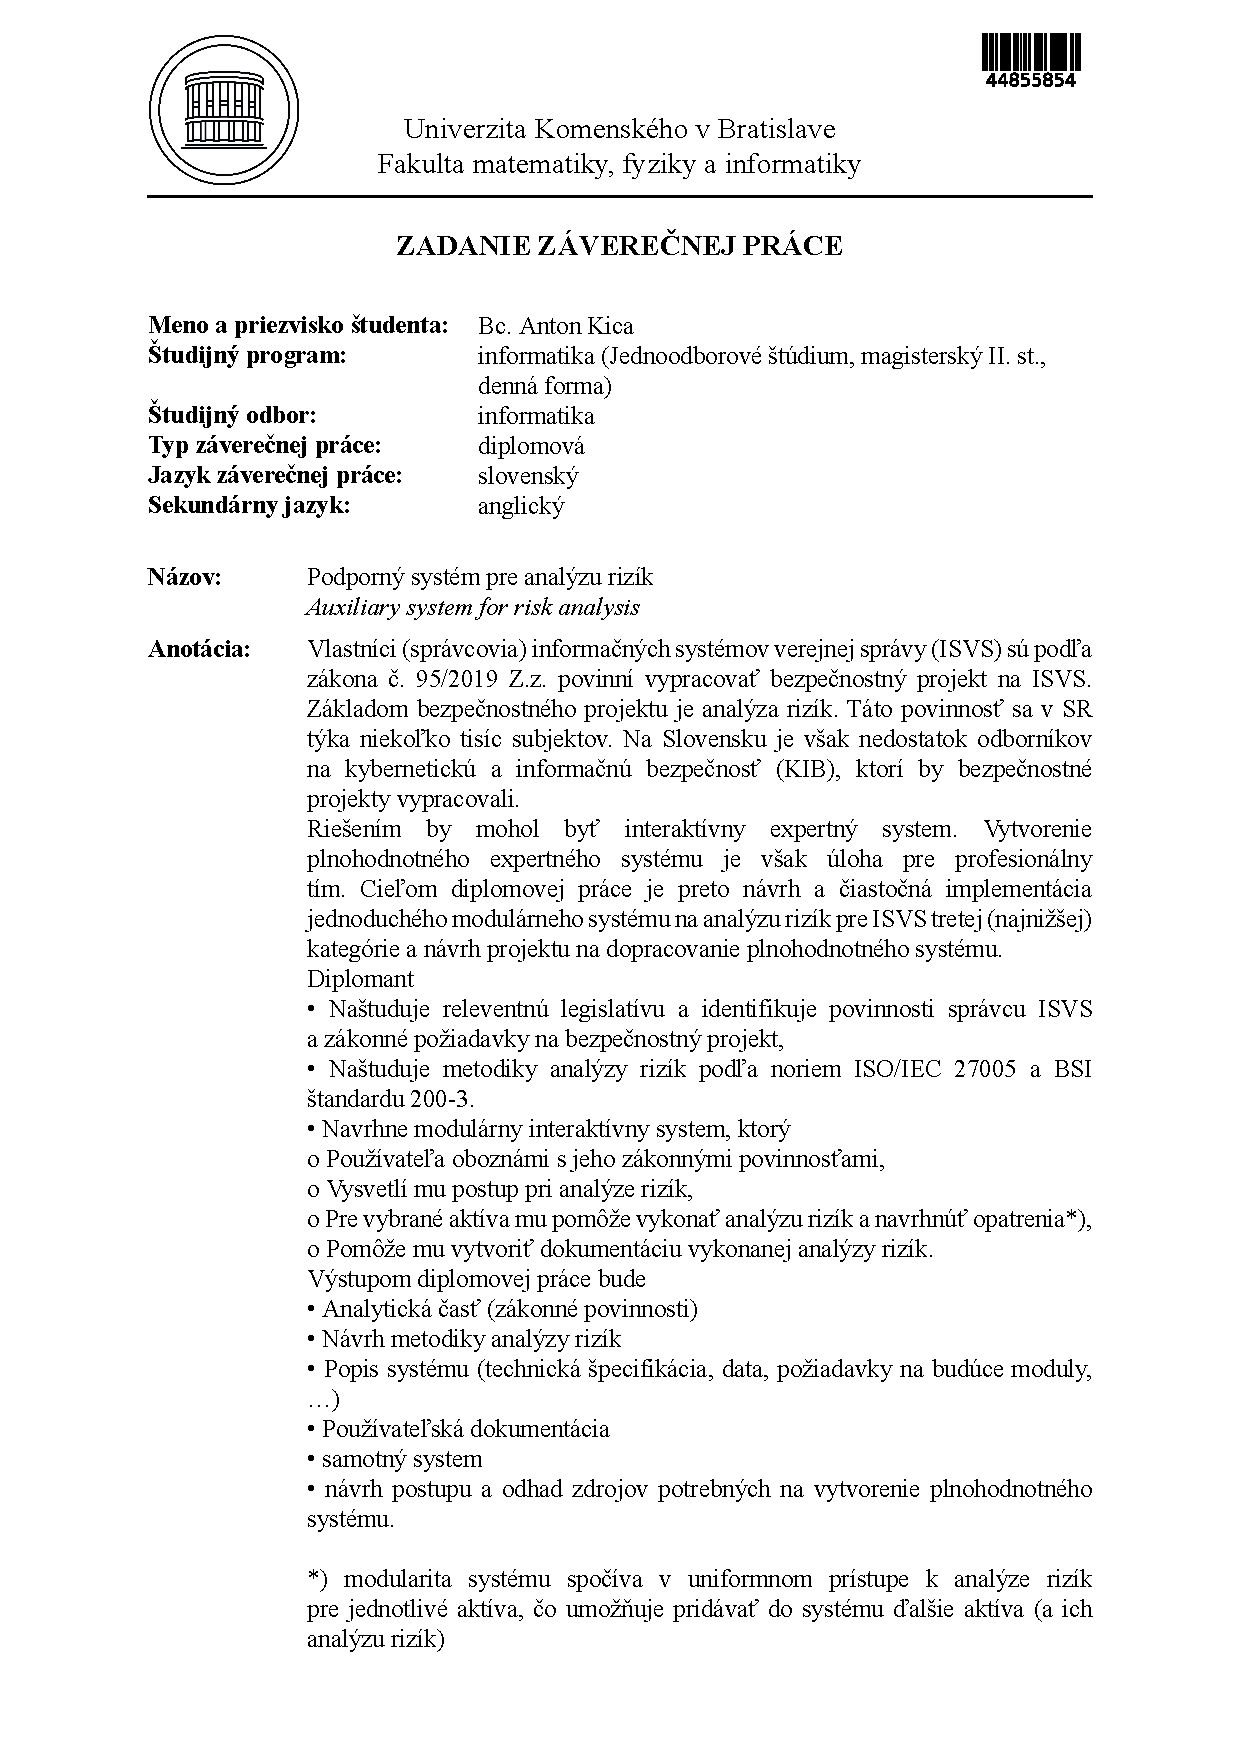
\includepdf[pages={1,2}]{images/zadanie.pdf}

% --- Koniec zadania


% -------------------
%   Čestné vyhlásenie a nepovinné poďakovanie
% -------------------
\newpage 
\pagestyle{plain}
\paragraph{Čestné vyhlásenie:}
Čestne vyhlasujem, že celú prácu na tému \uv{\mfnazov},
vrátane všetkých jej príloh a obrázkov, som vypracoval
samostatne, a to s použitím literatúry uvedenej v priloženom zozname.

% Uveďte na čo ste nástroje používali
% Podľa typu použitia potom nástroje aj citujte v texte
Pri príprave tejto práce boli tiež použité nástroje umelej inteligencie
\emph{Claude Opus 4.6} za účelom pomoci pri tvorbe TIKZ diagramov a grafiky a tiež na generovanie tzv. \emph{boilerplate} kódu.
Nástroje umelej inteligencie som použil v súlade s príslušnými právnymi
predpismi, akademickými právami a slobodami, etickými a morálnymi
zásadami za súčasného dodržania akademickej integrity. Som si
vedomý, že plne zodpovedám za správnosť výsledného textu.

\paragraph{Poďakovanie:} 
Ďakujem vedúcemu diplomovej práce doc. RNDr. Danielovi Olejárovi, PhD. za jeho cenné vedomosti, trpezlivosť, rady, pripomienky a študijné
materiály, ďakujem učiteľom a spolužiakom za inšpiratívne diskusie a ďakujem aj mojej rodine za ich nepretržitú podporu.
% -------------------
%   Abstrakt - Slovensky
% -------------------
\newpage 
\section*{Abstrakt}

Nemecké štandardy úradu BSI poskytujú systematický rámec na budovanie ISMS a praktický postup na vykonanie analýzy rizík. Cieľom našej práce
je navrhnúť podporný systém na analýzu rizík na základe Kompendia a štandardu BSI 200-3. V práci čitateľovi vysvetlíme ISMS; popíšeme proces
analýzy rizík; analyzujeme, navrhneme a implementujeme pomocný systém na analýzu rizík; a nakoniec zhrnieme
problémy a východiska pre ďalšiu prácu. Výsledkom je \emph{proof-of-concept} implementácia systému na podporu analýzy rizík, ktorá cez webové
rozhranie uchováva informácie do databázy určené na ďalšie spracovanie. 



\paragraph*{Kľúčové slová:}
% --- Koniec Abstrakt - Slovensky
analýza rizík, ISMS, BSI, KIB


% -------------------
% --- Abstrakt - Anglicky 
% -------------------
\newpage 
\section*{Abstract}
The German BSI standards provide a systematic framework for establishing an ISMS and a practical procedure for conducting a risk analysis.
The aim of our work is to design a support system for risk analysis based on the Compendium and the BSI 200-3 standard. In this work, we
explain ISMS to the reader; describe the risk analysis process; analyze, design, and implement a support system for risk
analysis; and finally summarize the challenges and directions for further work. The result is a \emph{proof-of-concept} implementation of
a system to support risk analysis, which stores information via a web interface into a database intended for further processing.

\paragraph*{Keywords:} 
risk analysis, ISMS, BSI, KIB

% --- Koniec Abstrakt - Anglicky


% -------------------
% --- Obsah
% -------------------


\cleardoublepage
\tableofcontents

% ---  Koniec Obsahu

% -------------------
% --- Zoznamy tabuliek, obrázkov, skratiek, slovník - nepovinné
% -------------------

\newpage 

\listoffigures
\listoftables

% ---  Koniec Zoznamov

\mainmatter
\pagestyle{headings}


\input 00_uvod.tex 
\input 10_terms.tex 
\input 11_it_grundschutz.tex 
\input 12_analyzarizik.tex 
\input 13_aplikacia.tex 
\input 14_future_works.tex 
\input 20_zaver.tex

% -------------------
% --- Bibliografia
% -------------------


\newpage	

\backmatter

\thispagestyle{empty}
\clearpage
\addcontentsline{toc}{chapter}{Literatúra}
\bibliographystyle{abstract}
\bibliography{literatura}

%---koniec Referencii

% -------------------
%--- Prilohy---
% -------------------

%Nepovinná časť prílohy obsahuje materiály, ktoré neboli zaradené priamo  do textu. Každá príloha sa začína na novej strane.
%Zoznam príloh je súčasťou obsahu.
%
\appendix
\chapter{Elektronická príloha}\label{chap:appendix}

Súčasťou elektronickej prílohy sú štyri súbory:
\begin{enumerate}[nosep,label=\alph*)]
    \item zdrojový kód pre backend
    \item zdrojový kód pre frontend
    \item užívateľská príručka systému
    \item kategorizácia základných hrozieb IT-Grundschutz podľa 27005
\end{enumerate}

\end{document}
